\hypertarget{implementation}{%
\section{\# Implementation}\label{implementation}}

\hypertarget{using-probabilistic-graphical-models-to-forecast-the-price-of-crude-oil}{%
\paragraph{(Using Probabilistic Graphical Models to forecast the price
of crude
oil)}\label{using-probabilistic-graphical-models-to-forecast-the-price-of-crude-oil}}

The document contains the \textbf{implementation} of the oil trading
system using graphical models.

\begin{itemize}
\tightlist
\item
  \protect\hyperlink{first}{The \textbf{first} part} is dedicated to
  retrieving data from the \textbf{EIA} and \textbf{FRED},
  \textbf{preprocessing} the data,and creating the \textbf{training},
  \textbf{validation}, and \textbf{test} datasets.
\item
  \protect\hyperlink{second}{The \textbf{second} part} is dedicated to
  implementing a \textbf{regime detection model} using \textbf{Hidden
  Markov Models} to identify bull, bear, and stagnant regimes
\item
  \protect\hyperlink{third}{The \textbf{third} part} is dedicated to
  learning the \textbf{macroeconomic structure} of the oil markets by
  \textbf{learning the belief network} using \textbf{hill-climbing}
  structural learning.
\item
  \protect\hyperlink{fourth}{The \textbf{fourth} part} is dedicated to
  \textbf{testing} the constructed model by simulating trades and taking
  positions based on those trades.
\end{itemize}

It is recommended to take look at the thesis documentation to understand
the basis on which we selected the macroeconomic economic data from the
EIA and FRED, and the theoretical context of the graphical models being
employed in our model.

We would be using a number of Python packages, such as
\href{http://pgmpy.org/}{pgmpy} and
\href{https://github.com/lopatovsky/HMMs}{hmms} throughout the notebook
and it is highly recommended that we take a deeper look at them as only
a specific and relevant functionality of those packages have been used
in our model.

\hypertarget{data-preprocessing}{%
\subsection{Data preprocessing}\label{data-preprocessing}}

Data preprocessing plays an important role in Machine Learning. Our data
preprocessing has four main steps; data retrieval, data cleaning, data
transformation, and data discretisation.

\hypertarget{data-retrieval}{%
\subsubsection{Data retrieval}\label{data-retrieval}}

The first step of constructing our model is to retrieve the data from
the open-data facilities. We have selected the \textbf{EIA} and
\textbf{FRED} as our primary data sources. Unfortunately, both these
open-data facilities do not provide Python packages to neatly retrieve
data in Python, so we will have to resort to using third-party APIs. For
the EIA, we are using
\href{https://github.com/mra1385/EIA-python/}{EIA-python}, and for the
FRED we are using \href{https://github.com/mortada/fredapi}{fredapi}.

Before beginning, we would be first be importing pandas and numpy, as
they are highly required in the entire data preprocessing section.

\begin{lstlisting}[language=Python]
import pandas as pd # pandas is an open source, data structures and data analysis tool in Python
import numpy as np  # numpy is a Python library supporting high-level mathematical functions on large multidimensional arrays
\end{lstlisting}

We would now be retrieving data, beginning with the EIA. Before
retrieving data from the EIA, we have to register with EIA's
\href{https://www.eia.gov/opendata/}{open-data facility}, in return of
which we shall recieve an API key, which is used as a passphrase to
access data from the EIA's datacenter.

\begin{lstlisting}[language=Python]
import eia # Importing the library
eia_key = "265d1f2178aaab3ceec3d364d9cc1d11"; # the API key we recieved from EIA
eia_api = eia.API(eia_key); # Initiates a session with the EIA datacenter to recieve datasets
\end{lstlisting}

Now, we shall be making a request to retrieve data from the EIA as a
pandas dataframe. EIA provides a 3,872 Short-Term Energy Outlook (STEO)
datasets, with short-term (2-year) forecasts of each dataset. These
datasets can be searched in EIAs
\href{https://www.eia.gov/opendata/qb.php}{query browse} facility, which
also offers a catalogue of different datasets sorted by relevance. Just
as an example to demonstrate, we would be retrieving the \textbf{Crude
Oil Exports, Monthly}, which has a Series ID `\textbf{TOTAL.COEXPUS.M}'.

\begin{lstlisting}[language=Python]
eia_data = pd.DataFrame(eia_api.data_by_series(series='TOTAL.COEXPUS.M')); # Convert to pandas dataframe
\end{lstlisting}

\hypertarget{data-cleaning}{%
\subsubsection{Data Cleaning}\label{data-cleaning}}

Taking a look at the dataframe, we can observe some evident
inconsistencies.

Firstly, the dataframe provided by the EIA is not of the standard format
\textbf{datetime}, which pandas indexing supports and provides extensive
facility to. We would be writing a function which makes the index a
\textbf{datetime} object so that we can convert the dataframe to a
\textbf{datetime}-index dataframe for more compatibility with pandas,
hmms, and pgmpy.

\begin{lstlisting}[language=Python]
import datetime # Using the datetime library

def convert_to_datetime(input):
            return datetime.datetime.strptime(input[:9], "%Y %m ").date();

eia_data.index = eia_data.index.map(convert_to_datetime); # Apply to entire index
eia_data.index = pd.to_datetime(eia_data.index); # Convert dataframe index to datetime64[ns] index
eia_data.columns = ['TOTAL.COEXPUS.M']; # pgmpy stores the column names as the variable name
\end{lstlisting}

The second issue are \textbf{holes} in the data i.e.~rows marked by a
`-' (a single dash). We would be replacing these dashes by
\textbf{np.nan} so that we can use pandas to fill in the holes. Usually
the prevalance of these holes is very rare, but just to be on the safe
side to ensure we can possibly download every dataset.

\begin{lstlisting}[language=Python]
eia_data.replace('-', np.nan, regex=True, inplace=True); # Replace the '-' with np.nan
eia_data.fillna(method='bfill', inplace=True); # Backward fill the holes, by filling them with the data infront.
\end{lstlisting}

Together, we can create a function carrying out the entire process so
that we can easily clean EIA data in one step.

\begin{lstlisting}[language=Python]
def clean_EIA(data):
            data.replace('-', np.nan, regex=True, inplace=True);
            data.fillna(method='bfill', inplace=True);
            
            data.index = data.index.map(convert_to_datetime);
            data.index = pd.to_datetime(data.index);
\end{lstlisting}

The dataframe is now a time series dataframe which could be plotted as a
time-series dataframe.

\begin{lstlisting}[language=Python]
import matplotlib.pyplot as plt

fig, ax = plt.subplots(figsize=(20,6));
ax.plot(eia_data);
\end{lstlisting}

Now, we shall be taking a look at the FRED data. Similar to
\href{https://github.com/mra1385/EIA-python/}{EIA-python}, the
\href{https://github.com/mortada/fredapi}{fredapi} requires us to
register with \href{https://research.stlouisfed.org/docs/api/fred/}{FRED
API} so that we can access data. We would download the \textbf{Spot
Crude Oil Price: West Texas Intermediate}, having the Series ID
`\textbf{WTISPLC}.'

\begin{lstlisting}[language=Python]
from fredapi import Fred

fred_key = "029c72315e9ec4eaf3e679ec3f6a2cb3"; # FRED API key
fred = Fred(api_key=fred_key); # Initiates a session with the FRED datacenter to recieve datasets

fred_data = pd.DataFrame(fred.get_series('WTISPLC'), columns=['WTISPLC']); # Retrieve data from FRED API
\end{lstlisting}

It is evident that the FRED, though still being a government
organization, has `ready-to-use' / `plug'n play' data of useable quality
compared to the EIA. Fortuntely, we will not be having to clean data
obtained from the FRED.

\hypertarget{constructing-the-training-validation-and-testing-datasets-data-transformation}{%
\subsubsection{Constructing the training, validation and testing
datasets (Data
transformation)}\label{constructing-the-training-validation-and-testing-datasets-data-transformation}}

As mentioned in the thesis, we need to divide our data in three
portions: the training dataset, the validation dataset, and the training
dataset. Given that we would be using a number of datasets from the FRED
and the EIA, we would have to amalgamate these datasets into one
dataframe and then slice the dataframe accordingly.

The train, validation, and test datasets are to be observed with a ratio
of \(80:10:10\), which is a popular ettiquette

The choice of datasets has been described in the thesis.

\begin{lstlisting}[language=Python]
# Dataset series ID from the EIA

datasets_eia  = [
    
                        'STEO.RGDPQ_NONOECD.M',
                        'STEO.RGDPQ_OECD.M',
    
                        'STEO.PAPR_NONOPEC.M',
                        'STEO.PAPR_OPEC.M',
    
                        'STEO.PATC_OECD.M',
                        'STEO.PATC_NON_OECD.M',
                
    
                        'STEO.COPRPUS.M',
                        'STEO.CORIPUS.M',
                        'PET.MCRIMXX2.M',
                        
                        'STEO.FOREX_WORLD.M',
    
                        'STEO.PASC_OECD_T3.M',
    
                        'STEO.COPS_OPEC.M',
                        'STEO.COPC_OPEC.M',
    
                        'STEO.T3_STCHANGE_OOECD.M',
                        'STEO.T3_STCHANGE_NOECD.M',
                ];

# Dataset series ID from the FRED

datasets_fred = [
                        'CPIENGSL',
                        'CAPG211S',
                        'CAPUTLG211S',
                        'IPG211S',
                        'IPG211111CN',
                        'INDPRO',
                        'IPN213111N',
                        'PCU211211',
                
                ];
\end{lstlisting}

To construct the training, validation, and testing datasets, we need to
first \textbf{concatenate} the datasets into one dataframe, and then
slice it.

\begin{lstlisting}[language=Python]
data_merge = []; # List of dataframes to be concatenated

# Adding EIA datasets 

for series_id in datasets_eia:
        df = pd.DataFrame(eia_api.data_by_series(series=series_id));
        clean_EIA(df);
        df.columns = [series_id];   
        data_merge.append(df);

# Adding FRED datasets 

for series_id in datasets_fred:
        df = pd.DataFrame(fred.get_series(series_id), columns=[series_id]);
        data_merge.append(df);
\end{lstlisting}

We have to create two additional columns; one which has the current
crude oil price, and the other for the price of crude oil next month
(forecast). This will be used to forecast the price of oil and hence
allow us to make buy/sell decisions based on that forecast.

\begin{lstlisting}[language=Python]
datasets = datasets_eia + datasets_fred + ['WTISPLC', 'forecast'];

current =  pd.DataFrame(fred.get_series('WTISPLC'), columns=['WTISPLC']);
forecast = pd.DataFrame(fred.get_series('WTISPLC').shift(-1), columns=['forecast']);

data_merge.append(current);
data_merge.append(forecast);
\end{lstlisting}

We have to amalgamate all datasets together in a single dataframe,
therefore we would use the pandas \textbf{concatenate} function. This
would allow us to find the intersection of the date intervals of all
dataframes and construct a single dataframe on a common time interval.

\begin{lstlisting}[language=Python]
data = pd.concat(data_merge, axis=1, join='inner');
\end{lstlisting}

Slicing our dataframe in train, validation, and testing datasets,

\begin{lstlisting}[language=Python]
train_data = data[: int(data.shape[0] * 0.80)];
vald_data = data[int(0.80 * data.shape[0]) : int(0.90 * data.shape[0])];
test_data = data[int(0.90* data.shape[0]) : int(data.shape[0])];
\end{lstlisting}

\hypertarget{data-discretisation}{%
\subsubsection{Data Discretisation}\label{data-discretisation}}

The data we have collected is non-categorical data; it is unlabelled and
continuous. Belief networks have variables, each having discrete
\textbf{states}, and therefore we have to reduce our data from prices to
a set of states, such as bull, bear, and stagnant markets. In order to
detect these (hidden) states, we have to use graphical models called
\textbf{Hidden Markov Models}. The process of detecting hidden states in
time-series data is called \textbf{Regime Detection}.

\hypertarget{regime-detection}{%
\subsection{Regime Detection}\label{regime-detection}}

We would be using Python library called
\href{https://github.com/lopatovsky/HMMs}{hmms} for implementing the
\textbf{Hidden Markov Models}.

A \textbf{Hidden Markov Model} is a 5-tuple \((Q, \sum, \Pi, A, B)\),
where \(Q = \{q_{1}, \cdots, q_{N}\}\) is a finite set of
\(\mathcal{N}\) states, \(\sum = \{s_1, \cdots, s_{N}\}\) is the set of
\(\mathcal{M}\) possible symbols (emissions) in the language,
\(\Pi = \{\pi_{i}\}\) is the initial probability vector,
\(A = \{a_{ij}\}\) is the state transition probability matrix, and
\(B = \{b_i(v_k)\}\) is the emission probability matrix. The HMM can be
denoted by \(\lambda = (\Pi, A, B)\).

For detecting regimes in time-series data, we would be using
\textbf{Hidden Markov Models}, with the difference between consecutive
months being the symbols \(\sum\) (1 - increase / 0 - decrease), the
hidden states, \(Q\) being the \textbf{bull}, \textbf{bear},
\textbf{stagnant} market regimes.

Let us use `\textbf{WTISPL}' (Spot Crude Oil Price: West Texas
Intermediate) of and try to identify regimes in the time series.

\begin{lstlisting}[language=Python]
import hmms
\end{lstlisting}

\begin{lstlisting}[language=Python]
price = train_data['WTISPLC'];
\end{lstlisting}

We will now try to transform the time series which represents the output
emissions, with \(1\) representing an increase in the price from the
previous month and \(0\) representing a decrease in the price of the
oil.

\begin{lstlisting}[language=Python]
price_diff = price.diff()[1:]; # The first value is NaN as there is not a previous month to compare with
e_seq = np.array(price_diff.apply(lambda x: 1 if x > 0 else 0).values); # Replacing the change with 1 if positive, else 0
\end{lstlisting}

Given that we have obtained the output (observed emission sequence), we
can now use the \textbf{Baum-Welch algorithm} to learn the parameters of
the HMM generating this data.

We have earlier described the \textbf{Baum-Welch algorithm} in the
Background and Literature review, and we would be using the
implementation provided \href{https://github.com/lopatovsky/HMMs}{hmms}
to learn the parameters.

\textbf{IT IS VERY IMPORTANT} to note we can \textbf{only} use the
training data to train the HMM as we are assuming to be blind to the
testing data. However, we would be observing predictions on the
validation dataset and will tune our model to fit it, and we would be
using the testing dataframe to test the final performance of the tuned
model after validation.

We will create a model with random parameters, that will be eventually
trained to match the data - a discrete time HMM of three hidden states
(bull, bear, or stagnant) and two output variables (increase or
decrease).

\begin{lstlisting}[language=Python]
dhmm_r = hmms.DtHMM.random(3 , 2); 
\end{lstlisting}

Given that the \(\texttt{hmms.DtHMM}\) takes a list of arrays no creater
than length \(32\), we will have to split our array in arrays each of
length \(32\) or less.

\begin{lstlisting}[language=Python]
e_seq = np.array_split(e_seq, 32);
\end{lstlisting}

\hypertarget{baum-welch-algorithm}{%
\subsubsection{Baum-Welch Algorithm}\label{baum-welch-algorithm}}

We would now be using the \textbf{Baum-Welch algorithm} to learn the
parameters of the HMM generating the time-series.

The probability of the reestimated model after each iteration should
ideally be closer that the (unknown) generator's model, however chances
might be the estimation fell in the local optima.

Unfortunately, the financial time-series data do not have fixed
parameters, so the HMM has to be trained everytime when live-trading,
when using the \textbf{k-fold cross-validation} training method.

\begin{lstlisting}[language=Python]
dhmm_r.baum_welch(e_seq, 100); # 100 iterations
\end{lstlisting}

\begin{lstlisting}
iteration  1 / 100
iteration  2 / 100
iteration  3 / 100
iteration  4 / 100
iteration  5 / 100
iteration  6 / 100
iteration  7 / 100
iteration  8 / 100
iteration  9 / 100
iteration  10 / 100
iteration  11 / 100
iteration  12 / 100
iteration  13 / 100
iteration  14 / 100
iteration  15 / 100
iteration  16 / 100
iteration  17 / 100
iteration  18 / 100
iteration  19 / 100
iteration  20 / 100
iteration  21 / 100
iteration  22 / 100
iteration  23 / 100
iteration  24 / 100
iteration  25 / 100
iteration  26 / 100
iteration  27 / 100
iteration  28 / 100
iteration  29 / 100
iteration  30 / 100
iteration  31 / 100
iteration  32 / 100
iteration  33 / 100
iteration  34 / 100
iteration  35 / 100
iteration  36 / 100
iteration  37 / 100
iteration  38 / 100
iteration  39 / 100
iteration  40 / 100
iteration  41 / 100
iteration  42 / 100
iteration  43 / 100
iteration  44 / 100
iteration  45 / 100
iteration  46 / 100
iteration  47 / 100
iteration  48 / 100
iteration  49 / 100
iteration  50 / 100
iteration  51 / 100
iteration  52 / 100
iteration  53 / 100
iteration  54 / 100
iteration  55 / 100
iteration  56 / 100
iteration  57 / 100
iteration  58 / 100
iteration  59 / 100
iteration  60 / 100
iteration  61 / 100
iteration  62 / 100
iteration  63 / 100
iteration  64 / 100
iteration  65 / 100
iteration  66 / 100
iteration  67 / 100
iteration  68 / 100
iteration  69 / 100
iteration  70 / 100
iteration  71 / 100
iteration  72 / 100
iteration  73 / 100
iteration  74 / 100
iteration  75 / 100
iteration  76 / 100
iteration  77 / 100
iteration  78 / 100
iteration  79 / 100
iteration  80 / 100
iteration  81 / 100
iteration  82 / 100
iteration  83 / 100
iteration  84 / 100
iteration  85 / 100
iteration  86 / 100
iteration  87 / 100
iteration  88 / 100
iteration  89 / 100
iteration  90 / 100
iteration  91 / 100
iteration  92 / 100
iteration  93 / 100
iteration  94 / 100
iteration  95 / 100
iteration  96 / 100
iteration  97 / 100
iteration  98 / 100
iteration  99 / 100
iteration  100 / 100
\end{lstlisting}

We have now learnt the parameters generating the emission sequence.

\begin{lstlisting}[language=Python]
hmms.print_parameters( dhmm_r );
\end{lstlisting}

\begin{lstlisting}
Initial probabilities (π) :
\end{lstlisting}

0

0

0.695329

1

0.177620

2

0.127051

Transition probabilities matrix (A):

0

1

2

0

0.572717

0.359354

0.067928

1

0.085750

0.372324

0.541926

2

0.784855

0.158842

0.056303

Emission probabilities matrix (B):

0

1

0

0.090503

0.909497

1

0.971681

0.028319

2

0.240093

0.759907

\hypertarget{viterbi-algorithm}{%
\subsubsection{Viterbi Algorithm}\label{viterbi-algorithm}}

Now, given we now have parameters \(\lambda\) and the emitted
observation sequence \(\texttt{e_seq}\), we can use the \textbf{Viterbi
Algorithm} to identify the most likely \textbf{state-transition} path
(i.e. \textbf{market regimes}) in the financial time-series.

\begin{lstlisting}[language=Python]
( log_prob, s_seq ) =  dhmm_r.viterbi(np.concatenate(e_seq).ravel());
\end{lstlisting}

\hypertarget{multicolored-time-series-plot}{%
\subsubsection{Multicolored time series
plot}\label{multicolored-time-series-plot}}

Now, we will be plotting this graph in a \textbf{multicolored}
time-series plot to observe how well the regimes have been identified.

First, we will have to make a dataframe which has the both the price and
the associated regime the time-series data is in.

\begin{lstlisting}[language=Python]
price_plot = pd.DataFrame(price[1:], index=price[1:].index); # Add price
price_plot['Regime'] = s_seq; # Add a column representing the regime 
price_plot['diff'] = price_diff; # Add a column representing the increase or decrease in price
\end{lstlisting}

We do not know, however, which state represents which regime. Given that
the bull regimes should have a high positive change in price, bear
regimes should have a high negative change, and stagnant regimes are
closer to zero, we can use these properties to tell which state
represents which regime.

\begin{lstlisting}[language=Python]
means = price_plot.groupby(['Regime'])['diff'].mean(); # Get means of all assigned states
lst_1 = means.index.tolist();
lst_2 = means.sort_values().index.tolist();

map_regimes = dict(zip(lst_2, lst_1));

price_plot['Regime'] = price_plot['Regime'].map(map_regimes);
\end{lstlisting}

Plotting the data as \textbf{multi-colored} time series:

\begin{lstlisting}[language=Python]
import matplotlib.dates as mdates
import matplotlib.patches as mpatches
from matplotlib.collections import LineCollection
from matplotlib.colors import Colormap, ListedColormap, BoundaryNorm

fig, ax1 = plt.subplots(figsize=(20,8));
ax.plot(price_plot['WTISPLC']);

cmap   = ListedColormap(['r','b','g'],'indexed'); # Make 0 (Bear) - red, 1 (Stagnant) - blue, 2 (Bull) - green 
norm   = BoundaryNorm(range(3 + 1), cmap.N);
inxval = mdates.date2num(price_plot['WTISPLC'].index.to_pydatetime());
points = np.array([inxval, price_plot['WTISPLC']]).T.reshape(-1, 1, 2);
segments = np.concatenate([points[:-1], points[1:]], axis=1);

lc = LineCollection(segments, cmap=cmap, norm=norm);
lc.set_array(price_plot['Regime']);
plt.gca().add_collection(lc);
plt.xlim(price_plot['WTISPLC'].index.min(), price_plot['WTISPLC'].index.max());
plt.ylim(price_plot['WTISPLC'].min(), price_plot['WTISPLC'].max());

r_patch = mpatches.Patch(color='red', label='Bear');
g_patch = mpatches.Patch(color='green', label='Bull');
b_patch = mpatches.Patch(color='blue', label='Stagnant');

plt.legend(handles=[r_patch, g_patch, b_patch]);

plt.show();
\end{lstlisting}

\begin{figure}
\centering
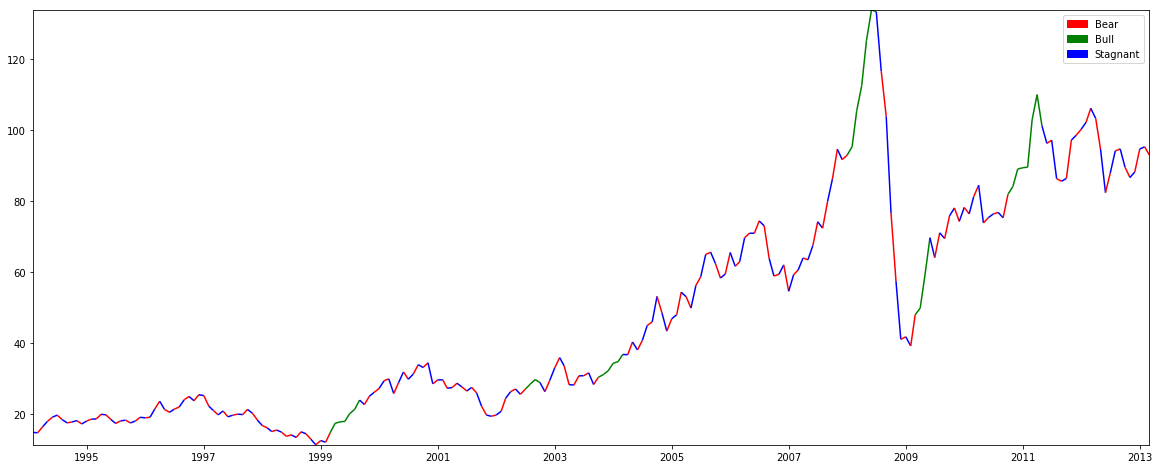
\includegraphics{Implementation_files/Implementation_49_0.png}
\caption{png}
\end{figure}

We can observe from the graph that there are periods of bear runs, bull
runs, and stagnant periods. Now, we need to apply a similar method to
all the training data so that we can discretise our data and use it as
an input to our belief network.

\hypertarget{discretising-dataframes-using-hidden-markov-models}{%
\subsubsection{Discretising dataframes using Hidden Markov
Models}\label{discretising-dataframes-using-hidden-markov-models}}

We will write a function that trains an HMM, identifies the sequence of
hidden states, and then constructs a dataframe of all the variables and
stores it as training dataset.

Now, we shall apply the same method to the entire training dataset so
that we can discretise it.

First, we shall learn all the parameters of Hidden Markov Models of all
the variables and store them.

\begin{lstlisting}[language=Python]
for series_id in datasets:
    if series_id == 'forecast':
        break;
    else:
        dhmm = hmms.DtHMM.random(3,2);
        data_diff =  train_data[series_id].diff()[1:];
        emit_seq = np.array_split(data_diff.apply(lambda x: 1 if x > 0 else 0).values, 32);
        dhmm.baum_welch(emit_seq, 100);
        path = "./hmms/" + series_id.replace(".", "_");
        dhmm.save_params(path);

# To retrain a specific dataset you were not satisfied with

# retrain_dataset = 'STEO.RGDPQ_NONOECD.M';
# dhmm = hmms.DtHMM.random(3,2);
# data_diff =  train_data[retrain_dataset].diff()[1:];
# emit_seq = np.array_split(data_diff.apply(lambda x: 1 if x > 0 else 0).values, 32);
# dhmm.baum_welch(emit_seq, 100);
# path = "./hmms/" + retrain_dataset.replace(".", "_");
# dhmm.save_params(path);

# Comment out the code above if you have already learnt HMMs and do not want to relearn them
\end{lstlisting}

iteration 1 / 100 iteration 2 / 100 iteration 3 / 100 iteration 4 / 100
iteration 5 / 100 iteration 6 / 100 iteration 7 / 100 iteration 8 / 100
iteration 9 / 100 iteration 10 / 100 iteration 11 / 100 iteration 12 /
100 iteration 13 / 100 iteration 14 / 100 iteration 15 / 100 iteration
16 / 100 iteration 17 / 100 iteration 18 / 100 iteration 19 / 100
iteration 20 / 100 iteration 21 / 100 iteration 22 / 100 iteration 23 /
100 iteration 24 / 100 iteration 25 / 100 iteration 26 / 100 iteration
27 / 100 iteration 28 / 100 iteration 29 / 100 iteration 30 / 100
iteration 31 / 100 iteration 32 / 100 iteration 33 / 100 iteration 34 /
100 iteration 35 / 100 iteration 36 / 100 iteration 37 / 100 iteration
38 / 100 iteration 39 / 100 iteration 40 / 100 iteration 41 / 100
iteration 42 / 100 iteration 43 / 100 iteration 44 / 100 iteration 45 /
100 iteration 46 / 100 iteration 47 / 100 iteration 48 / 100 iteration
49 / 100 iteration 50 / 100 iteration 51 / 100 iteration 52 / 100
iteration 53 / 100 iteration 54 / 100 iteration 55 / 100 iteration 56 /
100 iteration 57 / 100 iteration 58 / 100 iteration 59 / 100 iteration
60 / 100 iteration 61 / 100 iteration 62 / 100 iteration 63 / 100
iteration 64 / 100 iteration 65 / 100 iteration 66 / 100 iteration 67 /
100 iteration 68 / 100 iteration 69 / 100 iteration 70 / 100 iteration
71 / 100 iteration 72 / 100 iteration 73 / 100 iteration 74 / 100
iteration 75 / 100 iteration 76 / 100 iteration 77 / 100 iteration 78 /
100 iteration 79 / 100 iteration 80 / 100 iteration 81 / 100 iteration
82 / 100 iteration 83 / 100 iteration 84 / 100 iteration 85 / 100
iteration 86 / 100 iteration 87 / 100 iteration 88 / 100 iteration 89 /
100 iteration 90 / 100 iteration 91 / 100 iteration 92 / 100 iteration
93 / 100 iteration 94 / 100 iteration 95 / 100 iteration 96 / 100
iteration 97 / 100 iteration 98 / 100 iteration 99 / 100 iteration 100 /
100 iteration 1 / 100 iteration 2 / 100 iteration 3 / 100 iteration 4 /
100 iteration 5 / 100 iteration 6 / 100 iteration 7 / 100 iteration 8 /
100 iteration 9 / 100 iteration 10 / 100 iteration 11 / 100 iteration 12
/ 100 iteration 13 / 100 iteration 14 / 100 iteration 15 / 100 iteration
16 / 100 iteration 17 / 100 iteration 18 / 100 iteration 19 / 100
iteration 20 / 100 iteration 21 / 100 iteration 22 / 100 iteration 23 /
100 iteration 24 / 100 iteration 25 / 100 iteration 26 / 100 iteration
27 / 100 iteration 28 / 100 iteration 29 / 100 iteration 30 / 100
iteration 31 / 100 iteration 32 / 100 iteration 33 / 100 iteration 34 /
100 iteration 35 / 100 iteration 36 / 100 iteration 37 / 100 iteration
38 / 100 iteration 39 / 100 iteration 40 / 100 iteration 41 / 100
iteration 42 / 100 iteration 43 / 100 iteration 44 / 100 iteration 45 /
100 iteration 46 / 100 iteration 47 / 100 iteration 48 / 100 iteration
49 / 100 iteration 50 / 100 iteration 51 / 100 iteration 52 / 100
iteration 53 / 100 iteration 54 / 100 iteration 55 / 100 iteration 56 /
100 iteration 57 / 100 iteration 58 / 100 iteration 59 / 100 iteration
60 / 100 iteration 61 / 100 iteration 62 / 100 iteration 63 / 100
iteration 64 / 100 iteration 65 / 100 iteration 66 / 100 iteration 67 /
100 iteration 68 / 100 iteration 69 / 100 iteration 70 / 100 iteration
71 / 100 iteration 72 / 100 iteration 73 / 100 iteration 74 / 100
iteration 75 / 100 iteration 76 / 100 iteration 77 / 100 iteration 78 /
100 iteration 79 / 100 iteration 80 / 100 iteration 81 / 100 iteration
82 / 100 iteration 83 / 100 iteration 84 / 100 iteration 85 / 100
iteration 86 / 100 iteration 87 / 100 iteration 88 / 100 iteration 89 /
100 iteration 90 / 100 iteration 91 / 100 iteration 92 / 100 iteration
93 / 100 iteration 94 / 100 iteration 95 / 100 iteration 96 / 100
iteration 97 / 100 iteration 98 / 100 iteration 99 / 100 iteration 100 /
100 iteration 1 / 100 iteration 2 / 100 iteration 3 / 100 iteration 4 /
100 iteration 5 / 100 iteration 6 / 100 iteration 7 / 100 iteration 8 /
100 iteration 9 / 100 iteration 10 / 100 iteration 11 / 100 iteration 12
/ 100 iteration 13 / 100 iteration 14 / 100 iteration 15 / 100 iteration
16 / 100 iteration 17 / 100 iteration 18 / 100 iteration 19 / 100
iteration 20 / 100 iteration 21 / 100 iteration 22 / 100 iteration 23 /
100 iteration 24 / 100 iteration 25 / 100 iteration 26 / 100 iteration
27 / 100 iteration 28 / 100 iteration 29 / 100 iteration 30 / 100
iteration 31 / 100 iteration 32 / 100 iteration 33 / 100 iteration 34 /
100 iteration 35 / 100 iteration 36 / 100 iteration 37 / 100 iteration
38 / 100 iteration 39 / 100 iteration 40 / 100 iteration 41 / 100
iteration 42 / 100 iteration 43 / 100 iteration 44 / 100 iteration 45 /
100 iteration 46 / 100 iteration 47 / 100 iteration 48 / 100 iteration
49 / 100 iteration 50 / 100 iteration 51 / 100 iteration 52 / 100
iteration 53 / 100 iteration 54 / 100 iteration 55 / 100 iteration 56 /
100 iteration 57 / 100 iteration 58 / 100 iteration 59 / 100 iteration
60 / 100 iteration 61 / 100 iteration 62 / 100 iteration 63 / 100
iteration 64 / 100 iteration 65 / 100 iteration 66 / 100 iteration 67 /
100 iteration 68 / 100 iteration 69 / 100 iteration 70 / 100 iteration
71 / 100 iteration 72 / 100 iteration 73 / 100 iteration 74 / 100
iteration 75 / 100 iteration 76 / 100 iteration 77 / 100 iteration 78 /
100 iteration 79 / 100 iteration 80 / 100 iteration 81 / 100 iteration
82 / 100 iteration 83 / 100 iteration 84 / 100 iteration 85 / 100
iteration 86 / 100 iteration 87 / 100 iteration 88 / 100 iteration 89 /
100 iteration 90 / 100 iteration 91 / 100 iteration 92 / 100 iteration
93 / 100 iteration 94 / 100 iteration 95 / 100 iteration 96 / 100
iteration 97 / 100 iteration 98 / 100 iteration 99 / 100 iteration 100 /
100 iteration 1 / 100 iteration 2 / 100 iteration 3 / 100 iteration 4 /
100 iteration 5 / 100 iteration 6 / 100 iteration 7 / 100 iteration 8 /
100 iteration 9 / 100 iteration 10 / 100 iteration 11 / 100 iteration 12
/ 100 iteration 13 / 100 iteration 14 / 100 iteration 15 / 100 iteration
16 / 100 iteration 17 / 100 iteration 18 / 100 iteration 19 / 100
iteration 20 / 100 iteration 21 / 100 iteration 22 / 100 iteration 23 /
100 iteration 24 / 100 iteration 25 / 100 iteration 26 / 100 iteration
27 / 100 iteration 28 / 100 iteration 29 / 100 iteration 30 / 100
iteration 31 / 100 iteration 32 / 100 iteration 33 / 100 iteration 34 /
100 iteration 35 / 100 iteration 36 / 100 iteration 37 / 100 iteration
38 / 100 iteration 39 / 100 iteration 40 / 100 iteration 41 / 100
iteration 42 / 100 iteration 43 / 100 iteration 44 / 100 iteration 45 /
100 iteration 46 / 100 iteration 47 / 100 iteration 48 / 100 iteration
49 / 100 iteration 50 / 100 iteration 51 / 100 iteration 52 / 100
iteration 53 / 100 iteration 54 / 100 iteration 55 / 100 iteration 56 /
100 iteration 57 / 100 iteration 58 / 100 iteration 59 / 100 iteration
60 / 100 iteration 61 / 100 iteration 62 / 100 iteration 63 / 100
iteration 64 / 100 iteration 65 / 100 iteration 66 / 100 iteration 67 /
100 iteration 68 / 100 iteration 69 / 100 iteration 70 / 100 iteration
71 / 100 iteration 72 / 100 iteration 73 / 100 iteration 74 / 100
iteration 75 / 100 iteration 76 / 100 iteration 77 / 100 iteration 78 /
100 iteration 79 / 100 iteration 80 / 100 iteration 81 / 100 iteration
82 / 100 iteration 83 / 100 iteration 84 / 100 iteration 85 / 100
iteration 86 / 100 iteration 87 / 100 iteration 88 / 100 iteration 89 /
100 iteration 90 / 100 iteration 91 / 100 iteration 92 / 100 iteration
93 / 100 iteration 94 / 100 iteration 95 / 100 iteration 96 / 100
iteration 97 / 100 iteration 98 / 100 iteration 99 / 100 iteration 100 /
100 iteration 1 / 100 iteration 2 / 100 iteration 3 / 100 iteration 4 /
100 iteration 5 / 100 iteration 6 / 100 iteration 7 / 100 iteration 8 /
100 iteration 9 / 100 iteration 10 / 100 iteration 11 / 100 iteration 12
/ 100 iteration 13 / 100 iteration 14 / 100 iteration 15 / 100 iteration
16 / 100 iteration 17 / 100 iteration 18 / 100 iteration 19 / 100
iteration 20 / 100 iteration 21 / 100 iteration 22 / 100 iteration 23 /
100 iteration 24 / 100 iteration 25 / 100 iteration 26 / 100 iteration
27 / 100 iteration 28 / 100 iteration 29 / 100 iteration 30 / 100
iteration 31 / 100 iteration 32 / 100 iteration 33 / 100 iteration 34 /
100 iteration 35 / 100 iteration 36 / 100 iteration 37 / 100 iteration
38 / 100 iteration 39 / 100 iteration 40 / 100 iteration 41 / 100
iteration 42 / 100 iteration 43 / 100 iteration 44 / 100 iteration 45 /
100 iteration 46 / 100 iteration 47 / 100 iteration 48 / 100 iteration
49 / 100 iteration 50 / 100 iteration 51 / 100 iteration 52 / 100
iteration 53 / 100 iteration 54 / 100 iteration 55 / 100 iteration 56 /
100 iteration 57 / 100 iteration 58 / 100 iteration 59 / 100 iteration
60 / 100 iteration 61 / 100 iteration 62 / 100 iteration 63 / 100
iteration 64 / 100 iteration 65 / 100 iteration 66 / 100 iteration 67 /
100 iteration 68 / 100 iteration 69 / 100 iteration 70 / 100 iteration
71 / 100 iteration 72 / 100 iteration 73 / 100 iteration 74 / 100
iteration 75 / 100 iteration 76 / 100 iteration 77 / 100 iteration 78 /
100 iteration 79 / 100 iteration 80 / 100 iteration 81 / 100 iteration
82 / 100 iteration 83 / 100 iteration 84 / 100 iteration 85 / 100
iteration 86 / 100 iteration 87 / 100 iteration 88 / 100 iteration 89 /
100 iteration 90 / 100 iteration 91 / 100 iteration 92 / 100 iteration
93 / 100 iteration 94 / 100 iteration 95 / 100 iteration 96 / 100
iteration 97 / 100 iteration 98 / 100 iteration 99 / 100 iteration 100 /
100 iteration 1 / 100 iteration 2 / 100 iteration 3 / 100 iteration 4 /
100 iteration 5 / 100 iteration 6 / 100 iteration 7 / 100 iteration 8 /
100 iteration 9 / 100 iteration 10 / 100 iteration 11 / 100 iteration 12
/ 100 iteration 13 / 100 iteration 14 / 100 iteration 15 / 100 iteration
16 / 100 iteration 17 / 100 iteration 18 / 100 iteration 19 / 100
iteration 20 / 100 iteration 21 / 100 iteration 22 / 100 iteration 23 /
100 iteration 24 / 100 iteration 25 / 100 iteration 26 / 100 iteration
27 / 100 iteration 28 / 100 iteration 29 / 100 iteration 30 / 100
iteration 31 / 100 iteration 32 / 100 iteration 33 / 100 iteration 34 /
100 iteration 35 / 100 iteration 36 / 100 iteration 37 / 100 iteration
38 / 100 iteration 39 / 100 iteration 40 / 100 iteration 41 / 100
iteration 42 / 100 iteration 43 / 100 iteration 44 / 100 iteration 45 /
100 iteration 46 / 100 iteration 47 / 100 iteration 48 / 100 iteration
49 / 100 iteration 50 / 100 iteration 51 / 100 iteration 52 / 100
iteration 53 / 100 iteration 54 / 100 iteration 55 / 100 iteration 56 /
100 iteration 57 / 100 iteration 58 / 100 iteration 59 / 100 iteration
60 / 100 iteration 61 / 100 iteration 62 / 100 iteration 63 / 100
iteration 64 / 100 iteration 65 / 100 iteration 66 / 100 iteration 67 /
100 iteration 68 / 100 iteration 69 / 100 iteration 70 / 100 iteration
71 / 100 iteration 72 / 100 iteration 73 / 100 iteration 74 / 100
iteration 75 / 100 iteration 76 / 100 iteration 77 / 100 iteration 78 /
100 iteration 79 / 100 iteration 80 / 100 iteration 81 / 100 iteration
82 / 100 iteration 83 / 100 iteration 84 / 100 iteration 85 / 100
iteration 86 / 100 iteration 87 / 100 iteration 88 / 100 iteration 89 /
100 iteration 90 / 100 iteration 91 / 100 iteration 92 / 100 iteration
93 / 100 iteration 94 / 100 iteration 95 / 100 iteration 96 / 100
iteration 97 / 100 iteration 98 / 100 iteration 99 / 100 iteration 100 /
100 iteration 1 / 100 iteration 2 / 100 iteration 3 / 100 iteration 4 /
100 iteration 5 / 100 iteration 6 / 100 iteration 7 / 100 iteration 8 /
100 iteration 9 / 100 iteration 10 / 100 iteration 11 / 100 iteration 12
/ 100 iteration 13 / 100 iteration 14 / 100 iteration 15 / 100 iteration
16 / 100 iteration 17 / 100 iteration 18 / 100 iteration 19 / 100
iteration 20 / 100 iteration 21 / 100 iteration 22 / 100 iteration 23 /
100 iteration 24 / 100 iteration 25 / 100 iteration 26 / 100 iteration
27 / 100 iteration 28 / 100 iteration 29 / 100 iteration 30 / 100
iteration 31 / 100 iteration 32 / 100 iteration 33 / 100 iteration 34 /
100 iteration 35 / 100 iteration 36 / 100 iteration 37 / 100 iteration
38 / 100 iteration 39 / 100 iteration 40 / 100 iteration 41 / 100
iteration 42 / 100 iteration 43 / 100 iteration 44 / 100 iteration 45 /
100 iteration 46 / 100 iteration 47 / 100 iteration 48 / 100 iteration
49 / 100 iteration 50 / 100 iteration 51 / 100 iteration 52 / 100
iteration 53 / 100 iteration 54 / 100 iteration 55 / 100 iteration 56 /
100 iteration 57 / 100 iteration 58 / 100 iteration 59 / 100 iteration
60 / 100 iteration 61 / 100 iteration 62 / 100 iteration 63 / 100
iteration 64 / 100 iteration 65 / 100 iteration 66 / 100 iteration 67 /
100 iteration 68 / 100 iteration 69 / 100 iteration 70 / 100 iteration
71 / 100 iteration 72 / 100 iteration 73 / 100 iteration 74 / 100
iteration 75 / 100 iteration 76 / 100 iteration 77 / 100 iteration 78 /
100 iteration 79 / 100 iteration 80 / 100 iteration 81 / 100 iteration
82 / 100 iteration 83 / 100 iteration 84 / 100 iteration 85 / 100
iteration 86 / 100 iteration 87 / 100 iteration 88 / 100 iteration 89 /
100 iteration 90 / 100 iteration 91 / 100 iteration 92 / 100 iteration
93 / 100 iteration 94 / 100 iteration 95 / 100 iteration 96 / 100
iteration 97 / 100 iteration 98 / 100 iteration 99 / 100 iteration 100 /
100 iteration 1 / 100 iteration 2 / 100 iteration 3 / 100 iteration 4 /
100 iteration 5 / 100 iteration 6 / 100 iteration 7 / 100 iteration 8 /
100 iteration 9 / 100 iteration 10 / 100 iteration 11 / 100 iteration 12
/ 100 iteration 13 / 100 iteration 14 / 100 iteration 15 / 100 iteration
16 / 100 iteration 17 / 100 iteration 18 / 100 iteration 19 / 100
iteration 20 / 100 iteration 21 / 100 iteration 22 / 100 iteration 23 /
100 iteration 24 / 100 iteration 25 / 100 iteration 26 / 100 iteration
27 / 100 iteration 28 / 100 iteration 29 / 100 iteration 30 / 100
iteration 31 / 100 iteration 32 / 100 iteration 33 / 100 iteration 34 /
100 iteration 35 / 100 iteration 36 / 100 iteration 37 / 100 iteration
38 / 100 iteration 39 / 100 iteration 40 / 100 iteration 41 / 100
iteration 42 / 100 iteration 43 / 100 iteration 44 / 100 iteration 45 /
100 iteration 46 / 100 iteration 47 / 100 iteration 48 / 100 iteration
49 / 100 iteration 50 / 100 iteration 51 / 100 iteration 52 / 100
iteration 53 / 100 iteration 54 / 100 iteration 55 / 100 iteration 56 /
100 iteration 57 / 100 iteration 58 / 100 iteration 59 / 100 iteration
60 / 100 iteration 61 / 100 iteration 62 / 100 iteration 63 / 100
iteration 64 / 100 iteration 65 / 100 iteration 66 / 100 iteration 67 /
100 iteration 68 / 100 iteration 69 / 100 iteration 70 / 100 iteration
71 / 100 iteration 72 / 100 iteration 73 / 100 iteration 74 / 100
iteration 75 / 100 iteration 76 / 100 iteration 77 / 100 iteration 78 /
100 iteration 79 / 100 iteration 80 / 100 iteration 81 / 100 iteration
82 / 100 iteration 83 / 100 iteration 84 / 100 iteration 85 / 100
iteration 86 / 100 iteration 87 / 100 iteration 88 / 100 iteration 89 /
100 iteration 90 / 100 iteration 91 / 100 iteration 92 / 100 iteration
93 / 100 iteration 94 / 100 iteration 95 / 100 iteration 96 / 100
iteration 97 / 100 iteration 98 / 100 iteration 99 / 100 iteration 100 /
100 iteration 1 / 100 iteration 2 / 100 iteration 3 / 100 iteration 4 /
100 iteration 5 / 100 iteration 6 / 100 iteration 7 / 100 iteration 8 /
100 iteration 9 / 100 iteration 10 / 100 iteration 11 / 100 iteration 12
/ 100 iteration 13 / 100 iteration 14 / 100 iteration 15 / 100 iteration
16 / 100 iteration 17 / 100 iteration 18 / 100 iteration 19 / 100
iteration 20 / 100 iteration 21 / 100 iteration 22 / 100 iteration 23 /
100 iteration 24 / 100 iteration 25 / 100 iteration 26 / 100 iteration
27 / 100 iteration 28 / 100 iteration 29 / 100 iteration 30 / 100
iteration 31 / 100 iteration 32 / 100 iteration 33 / 100 iteration 34 /
100 iteration 35 / 100 iteration 36 / 100 iteration 37 / 100 iteration
38 / 100 iteration 39 / 100 iteration 40 / 100 iteration 41 / 100
iteration 42 / 100 iteration 43 / 100 iteration 44 / 100 iteration 45 /
100 iteration 46 / 100 iteration 47 / 100 iteration 48 / 100 iteration
49 / 100 iteration 50 / 100 iteration 51 / 100 iteration 52 / 100
iteration 53 / 100 iteration 54 / 100 iteration 55 / 100 iteration 56 /
100 iteration 57 / 100 iteration 58 / 100 iteration 59 / 100 iteration
60 / 100 iteration 61 / 100 iteration 62 / 100 iteration 63 / 100
iteration 64 / 100 iteration 65 / 100 iteration 66 / 100 iteration 67 /
100 iteration 68 / 100 iteration 69 / 100 iteration 70 / 100 iteration
71 / 100 iteration 72 / 100 iteration 73 / 100 iteration 74 / 100
iteration 75 / 100 iteration 76 / 100 iteration 77 / 100 iteration 78 /
100 iteration 79 / 100 iteration 80 / 100 iteration 81 / 100 iteration
82 / 100 iteration 83 / 100 iteration 84 / 100 iteration 85 / 100
iteration 86 / 100 iteration 87 / 100 iteration 88 / 100 iteration 89 /
100 iteration 90 / 100 iteration 91 / 100 iteration 92 / 100 iteration
93 / 100 iteration 94 / 100 iteration 95 / 100 iteration 96 / 100
iteration 97 / 100 iteration 98 / 100 iteration 99 / 100 iteration 100 /
100 iteration 1 / 100 iteration 2 / 100 iteration 3 / 100 iteration 4 /
100 iteration 5 / 100 iteration 6 / 100 iteration 7 / 100 iteration 8 /
100 iteration 9 / 100 iteration 10 / 100 iteration 11 / 100 iteration 12
/ 100 iteration 13 / 100 iteration 14 / 100 iteration 15 / 100 iteration
16 / 100 iteration 17 / 100 iteration 18 / 100 iteration 19 / 100
iteration 20 / 100 iteration 21 / 100 iteration 22 / 100 iteration 23 /
100 iteration 24 / 100 iteration 25 / 100 iteration 26 / 100 iteration
27 / 100 iteration 28 / 100 iteration 29 / 100 iteration 30 / 100
iteration 31 / 100 iteration 32 / 100 iteration 33 / 100 iteration 34 /
100 iteration 35 / 100 iteration 36 / 100 iteration 37 / 100 iteration
38 / 100 iteration 39 / 100 iteration 40 / 100 iteration 41 / 100
iteration 42 / 100 iteration 43 / 100 iteration 44 / 100 iteration 45 /
100 iteration 46 / 100 iteration 47 / 100 iteration 48 / 100 iteration
49 / 100 iteration 50 / 100 iteration 51 / 100 iteration 52 / 100
iteration 53 / 100 iteration 54 / 100 iteration 55 / 100 iteration 56 /
100 iteration 57 / 100 iteration 58 / 100 iteration 59 / 100 iteration
60 / 100 iteration 61 / 100 iteration 62 / 100 iteration 63 / 100
iteration 64 / 100 iteration 65 / 100 iteration 66 / 100 iteration 67 /
100 iteration 68 / 100 iteration 69 / 100 iteration 70 / 100 iteration
71 / 100 iteration 72 / 100 iteration 73 / 100 iteration 74 / 100
iteration 75 / 100 iteration 76 / 100 iteration 77 / 100 iteration 78 /
100 iteration 79 / 100 iteration 80 / 100 iteration 81 / 100 iteration
82 / 100 iteration 83 / 100 iteration 84 / 100 iteration 85 / 100
iteration 86 / 100 iteration 87 / 100 iteration 88 / 100 iteration 89 /
100 iteration 90 / 100 iteration 91 / 100 iteration 92 / 100 iteration
93 / 100 iteration 94 / 100 iteration 95 / 100 iteration 96 / 100
iteration 97 / 100 iteration 98 / 100 iteration 99 / 100 iteration 100 /
100 iteration 1 / 100 iteration 2 / 100 iteration 3 / 100 iteration 4 /
100 iteration 5 / 100 iteration 6 / 100 iteration 7 / 100 iteration 8 /
100 iteration 9 / 100 iteration 10 / 100 iteration 11 / 100 iteration 12
/ 100 iteration 13 / 100 iteration 14 / 100 iteration 15 / 100 iteration
16 / 100 iteration 17 / 100 iteration 18 / 100 iteration 19 / 100
iteration 20 / 100 iteration 21 / 100 iteration 22 / 100 iteration 23 /
100 iteration 24 / 100 iteration 25 / 100 iteration 26 / 100 iteration
27 / 100 iteration 28 / 100 iteration 29 / 100 iteration 30 / 100
iteration 31 / 100 iteration 32 / 100 iteration 33 / 100 iteration 34 /
100 iteration 35 / 100 iteration 36 / 100 iteration 37 / 100 iteration
38 / 100 iteration 39 / 100 iteration 40 / 100 iteration 41 / 100
iteration 42 / 100 iteration 43 / 100 iteration 44 / 100 iteration 45 /
100 iteration 46 / 100 iteration 47 / 100 iteration 48 / 100 iteration
49 / 100 iteration 50 / 100 iteration 51 / 100 iteration 52 / 100
iteration 53 / 100 iteration 54 / 100 iteration 55 / 100 iteration 56 /
100 iteration 57 / 100 iteration 58 / 100 iteration 59 / 100 iteration
60 / 100 iteration 61 / 100 iteration 62 / 100 iteration 63 / 100
iteration 64 / 100 iteration 65 / 100 iteration 66 / 100 iteration 67 /
100 iteration 68 / 100 iteration 69 / 100 iteration 70 / 100 iteration
71 / 100 iteration 72 / 100 iteration 73 / 100 iteration 74 / 100
iteration 75 / 100 iteration 76 / 100 iteration 77 / 100 iteration 78 /
100 iteration 79 / 100 iteration 80 / 100 iteration 81 / 100 iteration
82 / 100 iteration 83 / 100 iteration 84 / 100 iteration 85 / 100
iteration 86 / 100 iteration 87 / 100 iteration 88 / 100 iteration 89 /
100 iteration 90 / 100 iteration 91 / 100 iteration 92 / 100 iteration
93 / 100 iteration 94 / 100 iteration 95 / 100 iteration 96 / 100
iteration 97 / 100 iteration 98 / 100 iteration 99 / 100 iteration 100 /
100 iteration 1 / 100 iteration 2 / 100 iteration 3 / 100 iteration 4 /
100 iteration 5 / 100 iteration 6 / 100 iteration 7 / 100 iteration 8 /
100 iteration 9 / 100 iteration 10 / 100 iteration 11 / 100 iteration 12
/ 100 iteration 13 / 100 iteration 14 / 100 iteration 15 / 100 iteration
16 / 100 iteration 17 / 100 iteration 18 / 100 iteration 19 / 100
iteration 20 / 100 iteration 21 / 100 iteration 22 / 100 iteration 23 /
100 iteration 24 / 100 iteration 25 / 100 iteration 26 / 100 iteration
27 / 100 iteration 28 / 100 iteration 29 / 100 iteration 30 / 100
iteration 31 / 100 iteration 32 / 100 iteration 33 / 100 iteration 34 /
100 iteration 35 / 100 iteration 36 / 100 iteration 37 / 100 iteration
38 / 100 iteration 39 / 100 iteration 40 / 100 iteration 41 / 100
iteration 42 / 100 iteration 43 / 100 iteration 44 / 100 iteration 45 /
100 iteration 46 / 100 iteration 47 / 100 iteration 48 / 100 iteration
49 / 100 iteration 50 / 100 iteration 51 / 100 iteration 52 / 100
iteration 53 / 100 iteration 54 / 100 iteration 55 / 100 iteration 56 /
100 iteration 57 / 100 iteration 58 / 100 iteration 59 / 100 iteration
60 / 100 iteration 61 / 100 iteration 62 / 100 iteration 63 / 100
iteration 64 / 100 iteration 65 / 100 iteration 66 / 100 iteration 67 /
100 iteration 68 / 100 iteration 69 / 100 iteration 70 / 100 iteration
71 / 100 iteration 72 / 100 iteration 73 / 100 iteration 74 / 100
iteration 75 / 100 iteration 76 / 100 iteration 77 / 100 iteration 78 /
100 iteration 79 / 100 iteration 80 / 100 iteration 81 / 100 iteration
82 / 100 iteration 83 / 100 iteration 84 / 100 iteration 85 / 100
iteration 86 / 100 iteration 87 / 100 iteration 88 / 100 iteration 89 /
100 iteration 90 / 100 iteration 91 / 100 iteration 92 / 100 iteration
93 / 100 iteration 94 / 100 iteration 95 / 100 iteration 96 / 100
iteration 97 / 100 iteration 98 / 100 iteration 99 / 100 iteration 100 /
100 iteration 1 / 100 iteration 2 / 100 iteration 3 / 100 iteration 4 /
100 iteration 5 / 100 iteration 6 / 100 iteration 7 / 100 iteration 8 /
100 iteration 9 / 100 iteration 10 / 100 iteration 11 / 100 iteration 12
/ 100 iteration 13 / 100 iteration 14 / 100 iteration 15 / 100 iteration
16 / 100 iteration 17 / 100 iteration 18 / 100 iteration 19 / 100
iteration 20 / 100 iteration 21 / 100 iteration 22 / 100 iteration 23 /
100 iteration 24 / 100 iteration 25 / 100 iteration 26 / 100 iteration
27 / 100 iteration 28 / 100 iteration 29 / 100 iteration 30 / 100
iteration 31 / 100 iteration 32 / 100 iteration 33 / 100 iteration 34 /
100 iteration 35 / 100 iteration 36 / 100 iteration 37 / 100 iteration
38 / 100 iteration 39 / 100 iteration 40 / 100 iteration 41 / 100
iteration 42 / 100 iteration 43 / 100 iteration 44 / 100 iteration 45 /
100 iteration 46 / 100 iteration 47 / 100 iteration 48 / 100 iteration
49 / 100 iteration 50 / 100 iteration 51 / 100 iteration 52 / 100
iteration 53 / 100 iteration 54 / 100 iteration 55 / 100 iteration 56 /
100 iteration 57 / 100 iteration 58 / 100 iteration 59 / 100 iteration
60 / 100 iteration 61 / 100 iteration 62 / 100 iteration 63 / 100
iteration 64 / 100 iteration 65 / 100 iteration 66 / 100 iteration 67 /
100 iteration 68 / 100 iteration 69 / 100 iteration 70 / 100 iteration
71 / 100 iteration 72 / 100 iteration 73 / 100 iteration 74 / 100
iteration 75 / 100 iteration 76 / 100 iteration 77 / 100 iteration 78 /
100 iteration 79 / 100 iteration 80 / 100 iteration 81 / 100 iteration
82 / 100 iteration 83 / 100 iteration 84 / 100 iteration 85 / 100
iteration 86 / 100 iteration 87 / 100 iteration 88 / 100 iteration 89 /
100 iteration 90 / 100 iteration 91 / 100 iteration 92 / 100 iteration
93 / 100 iteration 94 / 100 iteration 95 / 100 iteration 96 / 100
iteration 97 / 100 iteration 98 / 100 iteration 99 / 100 iteration 100 /
100 iteration 1 / 100 iteration 2 / 100 iteration 3 / 100 iteration 4 /
100 iteration 5 / 100 iteration 6 / 100 iteration 7 / 100 iteration 8 /
100 iteration 9 / 100 iteration 10 / 100 iteration 11 / 100 iteration 12
/ 100 iteration 13 / 100 iteration 14 / 100 iteration 15 / 100 iteration
16 / 100 iteration 17 / 100 iteration 18 / 100 iteration 19 / 100
iteration 20 / 100 iteration 21 / 100 iteration 22 / 100 iteration 23 /
100 iteration 24 / 100 iteration 25 / 100 iteration 26 / 100 iteration
27 / 100 iteration 28 / 100 iteration 29 / 100 iteration 30 / 100
iteration 31 / 100 iteration 32 / 100 iteration 33 / 100 iteration 34 /
100 iteration 35 / 100 iteration 36 / 100 iteration 37 / 100 iteration
38 / 100 iteration 39 / 100 iteration 40 / 100 iteration 41 / 100
iteration 42 / 100 iteration 43 / 100 iteration 44 / 100 iteration 45 /
100 iteration 46 / 100 iteration 47 / 100 iteration 48 / 100 iteration
49 / 100 iteration 50 / 100 iteration 51 / 100 iteration 52 / 100
iteration 53 / 100 iteration 54 / 100 iteration 55 / 100 iteration 56 /
100 iteration 57 / 100 iteration 58 / 100 iteration 59 / 100 iteration
60 / 100 iteration 61 / 100 iteration 62 / 100 iteration 63 / 100
iteration 64 / 100 iteration 65 / 100 iteration 66 / 100 iteration 67 /
100 iteration 68 / 100 iteration 69 / 100 iteration 70 / 100 iteration
71 / 100 iteration 72 / 100 iteration 73 / 100 iteration 74 / 100
iteration 75 / 100 iteration 76 / 100 iteration 77 / 100 iteration 78 /
100 iteration 79 / 100 iteration 80 / 100 iteration 81 / 100 iteration
82 / 100 iteration 83 / 100 iteration 84 / 100 iteration 85 / 100
iteration 86 / 100 iteration 87 / 100 iteration 88 / 100 iteration 89 /
100 iteration 90 / 100 iteration 91 / 100 iteration 92 / 100 iteration
93 / 100 iteration 94 / 100 iteration 95 / 100 iteration 96 / 100
iteration 97 / 100 iteration 98 / 100 iteration 99 / 100 iteration 100 /
100 iteration 1 / 100 iteration 2 / 100 iteration 3 / 100 iteration 4 /
100 iteration 5 / 100 iteration 6 / 100 iteration 7 / 100 iteration 8 /
100 iteration 9 / 100 iteration 10 / 100 iteration 11 / 100 iteration 12
/ 100 iteration 13 / 100 iteration 14 / 100 iteration 15 / 100 iteration
16 / 100 iteration 17 / 100 iteration 18 / 100 iteration 19 / 100
iteration 20 / 100 iteration 21 / 100 iteration 22 / 100 iteration 23 /
100 iteration 24 / 100 iteration 25 / 100 iteration 26 / 100 iteration
27 / 100 iteration 28 / 100 iteration 29 / 100 iteration 30 / 100
iteration 31 / 100 iteration 32 / 100 iteration 33 / 100 iteration 34 /
100 iteration 35 / 100 iteration 36 / 100 iteration 37 / 100 iteration
38 / 100 iteration 39 / 100 iteration 40 / 100 iteration 41 / 100
iteration 42 / 100 iteration 43 / 100 iteration 44 / 100 iteration 45 /
100 iteration 46 / 100 iteration 47 / 100 iteration 48 / 100 iteration
49 / 100 iteration 50 / 100 iteration 51 / 100 iteration 52 / 100
iteration 53 / 100 iteration 54 / 100 iteration 55 / 100 iteration 56 /
100 iteration 57 / 100 iteration 58 / 100 iteration 59 / 100 iteration
60 / 100 iteration 61 / 100 iteration 62 / 100 iteration 63 / 100
iteration 64 / 100 iteration 65 / 100 iteration 66 / 100 iteration 67 /
100 iteration 68 / 100 iteration 69 / 100 iteration 70 / 100 iteration
71 / 100 iteration 72 / 100 iteration 73 / 100 iteration 74 / 100
iteration 75 / 100 iteration 76 / 100 iteration 77 / 100 iteration 78 /
100 iteration 79 / 100 iteration 80 / 100 iteration 81 / 100 iteration
82 / 100 iteration 83 / 100 iteration 84 / 100 iteration 85 / 100
iteration 86 / 100 iteration 87 / 100 iteration 88 / 100 iteration 89 /
100 iteration 90 / 100 iteration 91 / 100 iteration 92 / 100 iteration
93 / 100 iteration 94 / 100 iteration 95 / 100 iteration 96 / 100
iteration 97 / 100 iteration 98 / 100 iteration 99 / 100 iteration 100 /
100 iteration 1 / 100 iteration 2 / 100 iteration 3 / 100 iteration 4 /
100 iteration 5 / 100 iteration 6 / 100 iteration 7 / 100 iteration 8 /
100 iteration 9 / 100 iteration 10 / 100 iteration 11 / 100 iteration 12
/ 100 iteration 13 / 100 iteration 14 / 100 iteration 15 / 100 iteration
16 / 100 iteration 17 / 100 iteration 18 / 100 iteration 19 / 100
iteration 20 / 100 iteration 21 / 100 iteration 22 / 100 iteration 23 /
100 iteration 24 / 100 iteration 25 / 100 iteration 26 / 100 iteration
27 / 100 iteration 28 / 100 iteration 29 / 100 iteration 30 / 100
iteration 31 / 100 iteration 32 / 100 iteration 33 / 100 iteration 34 /
100 iteration 35 / 100 iteration 36 / 100 iteration 37 / 100 iteration
38 / 100 iteration 39 / 100 iteration 40 / 100 iteration 41 / 100
iteration 42 / 100 iteration 43 / 100 iteration 44 / 100 iteration 45 /
100 iteration 46 / 100 iteration 47 / 100 iteration 48 / 100 iteration
49 / 100 iteration 50 / 100 iteration 51 / 100 iteration 52 / 100
iteration 53 / 100 iteration 54 / 100 iteration 55 / 100 iteration 56 /
100 iteration 57 / 100 iteration 58 / 100 iteration 59 / 100 iteration
60 / 100 iteration 61 / 100 iteration 62 / 100 iteration 63 / 100
iteration 64 / 100 iteration 65 / 100 iteration 66 / 100 iteration 67 /
100 iteration 68 / 100 iteration 69 / 100 iteration 70 / 100 iteration
71 / 100 iteration 72 / 100 iteration 73 / 100 iteration 74 / 100
iteration 75 / 100 iteration 76 / 100 iteration 77 / 100 iteration 78 /
100 iteration 79 / 100 iteration 80 / 100 iteration 81 / 100 iteration
82 / 100 iteration 83 / 100 iteration 84 / 100 iteration 85 / 100
iteration 86 / 100 iteration 87 / 100 iteration 88 / 100 iteration 89 /
100 iteration 90 / 100 iteration 91 / 100 iteration 92 / 100 iteration
93 / 100 iteration 94 / 100 iteration 95 / 100 iteration 96 / 100
iteration 97 / 100 iteration 98 / 100 iteration 99 / 100 iteration 100 /
100 iteration 1 / 100 iteration 2 / 100 iteration 3 / 100 iteration 4 /
100 iteration 5 / 100 iteration 6 / 100 iteration 7 / 100 iteration 8 /
100 iteration 9 / 100 iteration 10 / 100 iteration 11 / 100 iteration 12
/ 100 iteration 13 / 100 iteration 14 / 100 iteration 15 / 100 iteration
16 / 100 iteration 17 / 100 iteration 18 / 100 iteration 19 / 100
iteration 20 / 100 iteration 21 / 100 iteration 22 / 100 iteration 23 /
100 iteration 24 / 100 iteration 25 / 100 iteration 26 / 100 iteration
27 / 100 iteration 28 / 100 iteration 29 / 100 iteration 30 / 100
iteration 31 / 100 iteration 32 / 100 iteration 33 / 100 iteration 34 /
100 iteration 35 / 100 iteration 36 / 100 iteration 37 / 100 iteration
38 / 100 iteration 39 / 100 iteration 40 / 100 iteration 41 / 100
iteration 42 / 100 iteration 43 / 100 iteration 44 / 100 iteration 45 /
100 iteration 46 / 100 iteration 47 / 100 iteration 48 / 100 iteration
49 / 100 iteration 50 / 100 iteration 51 / 100 iteration 52 / 100
iteration 53 / 100 iteration 54 / 100 iteration 55 / 100 iteration 56 /
100 iteration 57 / 100 iteration 58 / 100 iteration 59 / 100 iteration
60 / 100 iteration 61 / 100 iteration 62 / 100 iteration 63 / 100
iteration 64 / 100 iteration 65 / 100 iteration 66 / 100 iteration 67 /
100 iteration 68 / 100 iteration 69 / 100 iteration 70 / 100 iteration
71 / 100 iteration 72 / 100 iteration 73 / 100 iteration 74 / 100
iteration 75 / 100 iteration 76 / 100 iteration 77 / 100 iteration 78 /
100 iteration 79 / 100 iteration 80 / 100 iteration 81 / 100 iteration
82 / 100 iteration 83 / 100 iteration 84 / 100 iteration 85 / 100
iteration 86 / 100 iteration 87 / 100 iteration 88 / 100 iteration 89 /
100 iteration 90 / 100 iteration 91 / 100 iteration 92 / 100 iteration
93 / 100 iteration 94 / 100 iteration 95 / 100 iteration 96 / 100
iteration 97 / 100 iteration 98 / 100 iteration 99 / 100 iteration 100 /
100 iteration 1 / 100 iteration 2 / 100 iteration 3 / 100 iteration 4 /
100 iteration 5 / 100 iteration 6 / 100 iteration 7 / 100 iteration 8 /
100 iteration 9 / 100 iteration 10 / 100 iteration 11 / 100 iteration 12
/ 100 iteration 13 / 100 iteration 14 / 100 iteration 15 / 100 iteration
16 / 100 iteration 17 / 100 iteration 18 / 100 iteration 19 / 100
iteration 20 / 100 iteration 21 / 100 iteration 22 / 100 iteration 23 /
100 iteration 24 / 100 iteration 25 / 100 iteration 26 / 100 iteration
27 / 100 iteration 28 / 100 iteration 29 / 100 iteration 30 / 100
iteration 31 / 100 iteration 32 / 100 iteration 33 / 100 iteration 34 /
100 iteration 35 / 100 iteration 36 / 100 iteration 37 / 100 iteration
38 / 100 iteration 39 / 100 iteration 40 / 100 iteration 41 / 100
iteration 42 / 100 iteration 43 / 100 iteration 44 / 100 iteration 45 /
100 iteration 46 / 100 iteration 47 / 100 iteration 48 / 100 iteration
49 / 100 iteration 50 / 100 iteration 51 / 100 iteration 52 / 100
iteration 53 / 100 iteration 54 / 100 iteration 55 / 100 iteration 56 /
100 iteration 57 / 100 iteration 58 / 100 iteration 59 / 100 iteration
60 / 100 iteration 61 / 100 iteration 62 / 100 iteration 63 / 100
iteration 64 / 100 iteration 65 / 100 iteration 66 / 100 iteration 67 /
100 iteration 68 / 100 iteration 69 / 100 iteration 70 / 100 iteration
71 / 100 iteration 72 / 100 iteration 73 / 100 iteration 74 / 100
iteration 75 / 100 iteration 76 / 100 iteration 77 / 100 iteration 78 /
100 iteration 79 / 100 iteration 80 / 100 iteration 81 / 100 iteration
82 / 100 iteration 83 / 100 iteration 84 / 100 iteration 85 / 100
iteration 86 / 100 iteration 87 / 100 iteration 88 / 100 iteration 89 /
100 iteration 90 / 100 iteration 91 / 100 iteration 92 / 100 iteration
93 / 100 iteration 94 / 100 iteration 95 / 100 iteration 96 / 100
iteration 97 / 100 iteration 98 / 100 iteration 99 / 100 iteration 100 /
100 iteration 1 / 100 iteration 2 / 100 iteration 3 / 100 iteration 4 /
100 iteration 5 / 100 iteration 6 / 100 iteration 7 / 100 iteration 8 /
100 iteration 9 / 100 iteration 10 / 100 iteration 11 / 100 iteration 12
/ 100 iteration 13 / 100 iteration 14 / 100 iteration 15 / 100 iteration
16 / 100 iteration 17 / 100 iteration 18 / 100 iteration 19 / 100
iteration 20 / 100 iteration 21 / 100 iteration 22 / 100 iteration 23 /
100 iteration 24 / 100 iteration 25 / 100 iteration 26 / 100 iteration
27 / 100 iteration 28 / 100 iteration 29 / 100 iteration 30 / 100
iteration 31 / 100 iteration 32 / 100 iteration 33 / 100 iteration 34 /
100 iteration 35 / 100 iteration 36 / 100 iteration 37 / 100 iteration
38 / 100 iteration 39 / 100 iteration 40 / 100 iteration 41 / 100
iteration 42 / 100 iteration 43 / 100 iteration 44 / 100 iteration 45 /
100 iteration 46 / 100 iteration 47 / 100 iteration 48 / 100 iteration
49 / 100 iteration 50 / 100 iteration 51 / 100 iteration 52 / 100
iteration 53 / 100 iteration 54 / 100 iteration 55 / 100 iteration 56 /
100 iteration 57 / 100 iteration 58 / 100 iteration 59 / 100 iteration
60 / 100 iteration 61 / 100 iteration 62 / 100 iteration 63 / 100
iteration 64 / 100 iteration 65 / 100 iteration 66 / 100 iteration 67 /
100 iteration 68 / 100 iteration 69 / 100 iteration 70 / 100 iteration
71 / 100 iteration 72 / 100 iteration 73 / 100 iteration 74 / 100
iteration 75 / 100 iteration 76 / 100 iteration 77 / 100 iteration 78 /
100 iteration 79 / 100 iteration 80 / 100 iteration 81 / 100 iteration
82 / 100 iteration 83 / 100 iteration 84 / 100 iteration 85 / 100
iteration 86 / 100 iteration 87 / 100 iteration 88 / 100 iteration 89 /
100 iteration 90 / 100 iteration 91 / 100 iteration 92 / 100 iteration
93 / 100 iteration 94 / 100 iteration 95 / 100 iteration 96 / 100
iteration 97 / 100 iteration 98 / 100 iteration 99 / 100 iteration 100 /
100 iteration 1 / 100 iteration 2 / 100 iteration 3 / 100 iteration 4 /
100 iteration 5 / 100 iteration 6 / 100 iteration 7 / 100 iteration 8 /
100 iteration 9 / 100 iteration 10 / 100 iteration 11 / 100 iteration 12
/ 100 iteration 13 / 100 iteration 14 / 100 iteration 15 / 100 iteration
16 / 100 iteration 17 / 100 iteration 18 / 100 iteration 19 / 100
iteration 20 / 100 iteration 21 / 100 iteration 22 / 100 iteration 23 /
100 iteration 24 / 100 iteration 25 / 100 iteration 26 / 100 iteration
27 / 100 iteration 28 / 100 iteration 29 / 100 iteration 30 / 100
iteration 31 / 100 iteration 32 / 100 iteration 33 / 100 iteration 34 /
100 iteration 35 / 100 iteration 36 / 100 iteration 37 / 100 iteration
38 / 100 iteration 39 / 100 iteration 40 / 100 iteration 41 / 100
iteration 42 / 100 iteration 43 / 100 iteration 44 / 100 iteration 45 /
100 iteration 46 / 100 iteration 47 / 100 iteration 48 / 100 iteration
49 / 100 iteration 50 / 100 iteration 51 / 100 iteration 52 / 100
iteration 53 / 100 iteration 54 / 100 iteration 55 / 100 iteration 56 /
100 iteration 57 / 100 iteration 58 / 100 iteration 59 / 100 iteration
60 / 100 iteration 61 / 100 iteration 62 / 100 iteration 63 / 100
iteration 64 / 100 iteration 65 / 100 iteration 66 / 100 iteration 67 /
100 iteration 68 / 100 iteration 69 / 100 iteration 70 / 100 iteration
71 / 100 iteration 72 / 100 iteration 73 / 100 iteration 74 / 100
iteration 75 / 100 iteration 76 / 100 iteration 77 / 100 iteration 78 /
100 iteration 79 / 100 iteration 80 / 100 iteration 81 / 100 iteration
82 / 100 iteration 83 / 100 iteration 84 / 100 iteration 85 / 100
iteration 86 / 100 iteration 87 / 100 iteration 88 / 100 iteration 89 /
100 iteration 90 / 100 iteration 91 / 100 iteration 92 / 100 iteration
93 / 100 iteration 94 / 100 iteration 95 / 100 iteration 96 / 100
iteration 97 / 100 iteration 98 / 100 iteration 99 / 100 iteration 100 /
100 iteration 1 / 100 iteration 2 / 100 iteration 3 / 100 iteration 4 /
100 iteration 5 / 100 iteration 6 / 100 iteration 7 / 100 iteration 8 /
100 iteration 9 / 100 iteration 10 / 100 iteration 11 / 100 iteration 12
/ 100 iteration 13 / 100 iteration 14 / 100 iteration 15 / 100 iteration
16 / 100 iteration 17 / 100 iteration 18 / 100 iteration 19 / 100
iteration 20 / 100 iteration 21 / 100 iteration 22 / 100 iteration 23 /
100 iteration 24 / 100 iteration 25 / 100 iteration 26 / 100 iteration
27 / 100 iteration 28 / 100 iteration 29 / 100 iteration 30 / 100
iteration 31 / 100 iteration 32 / 100 iteration 33 / 100 iteration 34 /
100 iteration 35 / 100 iteration 36 / 100 iteration 37 / 100 iteration
38 / 100 iteration 39 / 100 iteration 40 / 100 iteration 41 / 100
iteration 42 / 100 iteration 43 / 100 iteration 44 / 100 iteration 45 /
100 iteration 46 / 100 iteration 47 / 100 iteration 48 / 100 iteration
49 / 100 iteration 50 / 100 iteration 51 / 100 iteration 52 / 100
iteration 53 / 100 iteration 54 / 100 iteration 55 / 100 iteration 56 /
100 iteration 57 / 100 iteration 58 / 100 iteration 59 / 100 iteration
60 / 100 iteration 61 / 100 iteration 62 / 100 iteration 63 / 100
iteration 64 / 100 iteration 65 / 100 iteration 66 / 100 iteration 67 /
100 iteration 68 / 100 iteration 69 / 100 iteration 70 / 100 iteration
71 / 100 iteration 72 / 100 iteration 73 / 100 iteration 74 / 100
iteration 75 / 100 iteration 76 / 100 iteration 77 / 100 iteration 78 /
100 iteration 79 / 100 iteration 80 / 100 iteration 81 / 100 iteration
82 / 100 iteration 83 / 100 iteration 84 / 100 iteration 85 / 100
iteration 86 / 100 iteration 87 / 100 iteration 88 / 100 iteration 89 /
100 iteration 90 / 100 iteration 91 / 100 iteration 92 / 100 iteration
93 / 100 iteration 94 / 100 iteration 95 / 100 iteration 96 / 100
iteration 97 / 100 iteration 98 / 100 iteration 99 / 100 iteration 100 /
100 iteration 1 / 100 iteration 2 / 100 iteration 3 / 100 iteration 4 /
100 iteration 5 / 100 iteration 6 / 100 iteration 7 / 100 iteration 8 /
100 iteration 9 / 100 iteration 10 / 100 iteration 11 / 100 iteration 12
/ 100 iteration 13 / 100 iteration 14 / 100 iteration 15 / 100 iteration
16 / 100 iteration 17 / 100 iteration 18 / 100 iteration 19 / 100
iteration 20 / 100 iteration 21 / 100 iteration 22 / 100 iteration 23 /
100 iteration 24 / 100 iteration 25 / 100 iteration 26 / 100 iteration
27 / 100 iteration 28 / 100 iteration 29 / 100 iteration 30 / 100
iteration 31 / 100 iteration 32 / 100 iteration 33 / 100 iteration 34 /
100 iteration 35 / 100 iteration 36 / 100 iteration 37 / 100 iteration
38 / 100 iteration 39 / 100 iteration 40 / 100 iteration 41 / 100
iteration 42 / 100 iteration 43 / 100 iteration 44 / 100 iteration 45 /
100 iteration 46 / 100 iteration 47 / 100 iteration 48 / 100 iteration
49 / 100 iteration 50 / 100 iteration 51 / 100 iteration 52 / 100
iteration 53 / 100 iteration 54 / 100 iteration 55 / 100 iteration 56 /
100 iteration 57 / 100 iteration 58 / 100 iteration 59 / 100 iteration
60 / 100 iteration 61 / 100 iteration 62 / 100 iteration 63 / 100
iteration 64 / 100 iteration 65 / 100 iteration 66 / 100 iteration 67 /
100 iteration 68 / 100 iteration 69 / 100 iteration 70 / 100 iteration
71 / 100 iteration 72 / 100 iteration 73 / 100 iteration 74 / 100
iteration 75 / 100 iteration 76 / 100 iteration 77 / 100 iteration 78 /
100 iteration 79 / 100 iteration 80 / 100 iteration 81 / 100 iteration
82 / 100 iteration 83 / 100 iteration 84 / 100 iteration 85 / 100
iteration 86 / 100 iteration 87 / 100 iteration 88 / 100 iteration 89 /
100 iteration 90 / 100 iteration 91 / 100 iteration 92 / 100 iteration
93 / 100 iteration 94 / 100 iteration 95 / 100 iteration 96 / 100
iteration 97 / 100 iteration 98 / 100 iteration 99 / 100 iteration 100 /
100 iteration 1 / 100 iteration 2 / 100 iteration 3 / 100 iteration 4 /
100 iteration 5 / 100 iteration 6 / 100 iteration 7 / 100 iteration 8 /
100 iteration 9 / 100 iteration 10 / 100 iteration 11 / 100 iteration 12
/ 100 iteration 13 / 100 iteration 14 / 100 iteration 15 / 100 iteration
16 / 100 iteration 17 / 100 iteration 18 / 100 iteration 19 / 100
iteration 20 / 100 iteration 21 / 100 iteration 22 / 100 iteration 23 /
100 iteration 24 / 100 iteration 25 / 100 iteration 26 / 100 iteration
27 / 100 iteration 28 / 100 iteration 29 / 100 iteration 30 / 100
iteration 31 / 100 iteration 32 / 100 iteration 33 / 100 iteration 34 /
100 iteration 35 / 100 iteration 36 / 100 iteration 37 / 100 iteration
38 / 100 iteration 39 / 100 iteration 40 / 100 iteration 41 / 100
iteration 42 / 100 iteration 43 / 100 iteration 44 / 100 iteration 45 /
100 iteration 46 / 100 iteration 47 / 100 iteration 48 / 100 iteration
49 / 100 iteration 50 / 100 iteration 51 / 100 iteration 52 / 100
iteration 53 / 100 iteration 54 / 100 iteration 55 / 100 iteration 56 /
100 iteration 57 / 100 iteration 58 / 100 iteration 59 / 100 iteration
60 / 100 iteration 61 / 100 iteration 62 / 100 iteration 63 / 100
iteration 64 / 100 iteration 65 / 100 iteration 66 / 100 iteration 67 /
100 iteration 68 / 100 iteration 69 / 100 iteration 70 / 100 iteration
71 / 100 iteration 72 / 100 iteration 73 / 100 iteration 74 / 100
iteration 75 / 100 iteration 76 / 100 iteration 77 / 100 iteration 78 /
100 iteration 79 / 100 iteration 80 / 100 iteration 81 / 100 iteration
82 / 100 iteration 83 / 100 iteration 84 / 100 iteration 85 / 100
iteration 86 / 100 iteration 87 / 100 iteration 88 / 100 iteration 89 /
100 iteration 90 / 100 iteration 91 / 100 iteration 92 / 100 iteration
93 / 100 iteration 94 / 100 iteration 95 / 100 iteration 96 / 100
iteration 97 / 100 iteration 98 / 100 iteration 99 / 100 iteration 100 /
100 iteration 1 / 100 iteration 2 / 100 iteration 3 / 100 iteration 4 /
100 iteration 5 / 100 iteration 6 / 100 iteration 7 / 100 iteration 8 /
100 iteration 9 / 100 iteration 10 / 100 iteration 11 / 100 iteration 12
/ 100 iteration 13 / 100 iteration 14 / 100 iteration 15 / 100 iteration
16 / 100 iteration 17 / 100 iteration 18 / 100 iteration 19 / 100
iteration 20 / 100 iteration 21 / 100 iteration 22 / 100 iteration 23 /
100 iteration 24 / 100 iteration 25 / 100 iteration 26 / 100 iteration
27 / 100 iteration 28 / 100 iteration 29 / 100 iteration 30 / 100
iteration 31 / 100 iteration 32 / 100 iteration 33 / 100 iteration 34 /
100 iteration 35 / 100 iteration 36 / 100 iteration 37 / 100 iteration
38 / 100 iteration 39 / 100 iteration 40 / 100 iteration 41 / 100
iteration 42 / 100 iteration 43 / 100 iteration 44 / 100 iteration 45 /
100 iteration 46 / 100 iteration 47 / 100 iteration 48 / 100 iteration
49 / 100 iteration 50 / 100 iteration 51 / 100 iteration 52 / 100
iteration 53 / 100 iteration 54 / 100 iteration 55 / 100 iteration 56 /
100 iteration 57 / 100 iteration 58 / 100 iteration 59 / 100 iteration
60 / 100 iteration 61 / 100 iteration 62 / 100 iteration 63 / 100
iteration 64 / 100 iteration 65 / 100 iteration 66 / 100 iteration 67 /
100 iteration 68 / 100 iteration 69 / 100 iteration 70 / 100 iteration
71 / 100 iteration 72 / 100 iteration 73 / 100 iteration 74 / 100
iteration 75 / 100 iteration 76 / 100 iteration 77 / 100 iteration 78 /
100 iteration 79 / 100 iteration 80 / 100 iteration 81 / 100 iteration
82 / 100 iteration 83 / 100 iteration 84 / 100 iteration 85 / 100
iteration 86 / 100 iteration 87 / 100 iteration 88 / 100 iteration 89 /
100 iteration 90 / 100 iteration 91 / 100 iteration 92 / 100 iteration
93 / 100 iteration 94 / 100 iteration 95 / 100 iteration 96 / 100
iteration 97 / 100 iteration 98 / 100 iteration 99 / 100 iteration 100 /
100

Now, we shall be constructing the discretised training dataframe.

\begin{lstlisting}[language=Python]
disc_test = pd.DataFrame(index = train_data[1:].index);

for series_id in datasets:
    path = "./hmms/" + series_id.replace(".", "_") + ".npz";
    if series_id == 'forecast':
        dhmm = hmms.DtHMM.from_file('./hmms/WTISPLC.npz');
    else:
        dhmm = hmms.DtHMM.from_file(path);
    data_diff =  train_data[series_id].diff()[1:];
    emit_seq = np.array(data_diff.apply(lambda x: 1 if x > 0 else 0).values);
    ( log_prob, s_seq ) =  dhmm.viterbi(emit_seq);
    disc_test[series_id] = s_seq;

disc_test.to_csv("./data/train_data.csv"); # Saving to CSV
\end{lstlisting}

\hypertarget{recommended-plotting-regime-switch-plots}{%
\subsubsection{(Recommended) Plotting Regime Switch
plots}\label{recommended-plotting-regime-switch-plots}}

In order to verify if the \textbf{HMM} has correctly identified regimes
in all datasets, we should plot the \textbf{regime-switching models} of
all datasets and observe if the \textbf{bull}, \textbf{bear}, and
\textbf{stagnant} states have been correctly identified. The graphical
representation allows us to understand how the regimes have been learnt.

Omission of this step can result in the \textbf{HMM} being incorrectly
trained, hence identifying incorrect regimes consequently affecting the
belief network's training and prediction process.

\begin{lstlisting}[language=Python]
states = pd.read_csv("./data/train_data.csv", index_col=0);

for series_id in datasets:
    
        df = pd.DataFrame(index=train_data[1:].index);
        df[series_id] = train_data[series_id][1:];
        df['Diff'] = train_data[series_id].diff()[1:];
        df['Regime'] = states[series_id];
        
        means = df.groupby(['Regime'])['Diff'].mean(); # Get means of all assigned states
        lst_1 = means.index.tolist();
        lst_2 = means.sort_values().index.tolist();

        map_regimes = dict(zip(lst_2, lst_1));
        df['Regime'] = df['Regime'].map(map_regimes);
        
        
        cmap   = ListedColormap(['r','b','g'],'indexed');
        norm   = BoundaryNorm(range(3 + 1), cmap.N);
        inxval = mdates.date2num(df[series_id].index.to_pydatetime());
        points = np.array([inxval, df[series_id]]).T.reshape(-1, 1, 2);
        segments = np.concatenate([points[:-1], points[1:]], axis=1);

        lc = LineCollection(segments, cmap=cmap, norm=norm);
        lc.set_array(df['Regime']);
        plt.gca().add_collection(lc);
        plt.xlim(df[series_id].index.min(), df[series_id].index.max());
        plt.ylim(df[series_id].min(), df[series_id].max());

        r_patch = mpatches.Patch(color='red', label='Bear');
        g_patch = mpatches.Patch(color='green', label='Bull');
        b_patch = mpatches.Patch(color='blue', label='Stagnant');

        plt.legend(handles=[r_patch, g_patch, b_patch]);

        name = "./plots/" + series_id.replace(".", "_") + ".png";

        plt.savefig(name);
        plt.close();
\end{lstlisting}

We have sucessfully discretised our training dataset and would now be
using it to train the Belief Network.

\hypertarget{learning-bayesian-network-using-hill-climbing}{%
\subsubsection{Learning Bayesian Network using Hill
Climbing}\label{learning-bayesian-network-using-hill-climbing}}

Given that we have discretised our training dataset, we can now use
\href{http://pgmpy.org/}{pgmpy} to construct a belief network of all the
variables.

We would be using the \textbf{Hill Climbing} approach to learn the
belief network. We have given a brief description of the Hill Climbing
algorithm in the thesis and would now be using its implementation pgmpy
to learn the structure of the oil markets.

We shall begin with importing the relevant modules from pgmpy in Python.

Given we would be using the \emph{BIC Scoring Algorithm} as the scoring
function for Hill Climbing, we will import the relevant functions from
the relevant module in pgmpy.

\begin{lstlisting}[language=Python]
from pgmpy.estimators import HillClimbSearch
from pgmpy.estimators import BayesianEstimator
from pgmpy.estimators import BicScore, K2Score, BdeuScore

train_data = pd.read_csv("./data/train_data.csv", index_col=0); # Retrieve training set
\end{lstlisting}

We shall now be performing a Hill-Climbing search. As difficult as it
seems, it is a quite straightforward process.

\begin{lstlisting}[language=Python]
hc = HillClimbSearch(train_data, scoring_method=BicScore(train_data)); #  Initialise Hill Climbing Estimator
model = hc.estimate(); # Performs local hill climb search

model.fit(train_data, 
          state_names=dict(map(lambda e: (e, [0, 1, 2]), datasets)), 
          estimator=BayesianEstimator, prior_type="BDeu");
\end{lstlisting}

\begin{lstlisting}[language=Python]
print(model.edges());
\end{lstlisting}

{[}(`STEO.RGDPQ\_NONOECD.M', `STEO.COPRPUS.M'), (`STEO.PATC\_OECD.M',
`STEO.PASC\_OECD\_T3.M'), (`STEO.FOREX\_WORLD.M', `STEO.COPC\_OPEC.M'),
(`STEO.PASC\_OECD\_T3.M', `STEO.T3\_STCHANGE\_OOECD.M'),
(`STEO.COPS\_OPEC.M', `STEO.PAPR\_OPEC.M'),
(`STEO.T3\_STCHANGE\_OOECD.M', `CAPUTLG211S'), (`CPIENGSL',
`PCU211211'), (`CAPUTLG211S', `STEO.PATC\_NON\_OECD.M'), (`WTISPLC',
`CPIENGSL'), (`forecast', `WTISPLC'){]}

We can also represent our model in the form of a directed graph, using
NetworkX.

\begin{lstlisting}[language=Python]
import networkx as nx
import matplotlib.pyplot as plt

G = nx.DiGraph();
G.add_edges_from(model.edges());
pos = nx.spring_layout(G)
nx.draw_networkx_edges(G, pos, node_size = 2000, arrows=True);
plt.show();
\end{lstlisting}

\begin{figure}
\centering
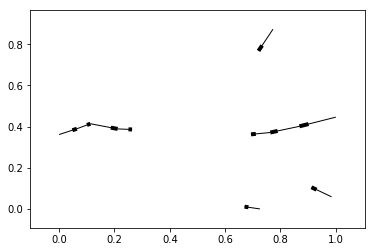
\includegraphics{Implementation_files/Implementation_64_0.png}
\caption{png}
\end{figure}

We have now fitted our model using the Hill Climb search, and now can
make inferences using forecasts as evidence.

\hypertarget{testing}{%
\subsection{Testing}\label{testing}}

We have successfully fitted our model to the data and need to test our
model now.

We will now be using our \textbf{validation} dataset and would be making
predictions on that and would be accordingly adjusting our model if we
are not satisfied by the performance.

We first have to discretise the validation dataset. We would be using
the HMMs trained on the \textbf{training set}. We \textbf{CANNOT} use
the \textbf{validation set} to train anything, including HMMs!

\begin{lstlisting}[language=Python]
discrete_vald = pd.DataFrame(index = vald_data[1:].index);

for series_id in datasets:
    path = "./hmms/" + series_id.replace(".", "_") + ".npz";
    if series_id == 'forecast':
        dhmm = hmms.DtHMM.from_file('./hmms/WTISPLC.npz');
    else:
        dhmm = hmms.DtHMM.from_file(path);
    data_diff =  vald_data[series_id].diff()[1:];
    emit_seq = np.array(data_diff.apply(lambda x: 1 if x > 0 else 0).values);
    ( log_prob, s_seq ) =  dhmm.viterbi(emit_seq);
    discrete_vald[series_id] = s_seq;

discrete_vald.to_csv("./data/validation_data.csv"); # Saving to CSV
\end{lstlisting}

Now, we shall be plotting this data to see how well the trained HMMs
predicted regimes on the valdiation dataset.

\begin{lstlisting}[language=Python]
states = pd.read_csv("./data/validation_data.csv", index_col=0);

for series_id in datasets:
    
        df = pd.DataFrame(index=vald_data[1:].index);
        df[series_id] = vald_data[series_id][1:];
        df['Diff'] = vald_data[series_id].diff()[1:];
        df['Regime'] = states[series_id];
        
        means = df.groupby(['Regime'])['Diff'].mean(); # Get means of all assigned states
        lst_1 = means.index.tolist();
        lst_2 = means.sort_values().index.tolist();

        map_regimes = dict(zip(lst_2, lst_1));
        df['Regime'] = df['Regime'].map(map_regimes);
        
        
        cmap   = ListedColormap(['r','b','g'],'indexed');
        norm   = BoundaryNorm(range(3 + 1), cmap.N);
        inxval = mdates.date2num(df[series_id].index.to_pydatetime());
        points = np.array([inxval, df[series_id]]).T.reshape(-1, 1, 2);
        segments = np.concatenate([points[:-1], points[1:]], axis=1);

        lc = LineCollection(segments, cmap=cmap, norm=norm);
        lc.set_array(df['Regime']);
        plt.gca().add_collection(lc);
        plt.xlim(df[series_id].index.min(), df[series_id].index.max());
        plt.ylim(df[series_id].min(), df[series_id].max());

        r_patch = mpatches.Patch(color='red', label='Bear');
        g_patch = mpatches.Patch(color='green', label='Bull');
        b_patch = mpatches.Patch(color='blue', label='Stagnant');

        plt.legend(handles=[r_patch, g_patch, b_patch]);

        name = "./plots/" + series_id.replace(".", "_") + "_VALIDATION.png";

        plt.savefig(name);
        plt.close();
\end{lstlisting}

Now, we would be predicting the validation sets (forecast for Spot Crude
Oil price, WTI Monthly).

For that, we have to drop the forecast column and then do an inference
on the model.

\begin{lstlisting}[language=Python]
vald_real = states['WTISPLC'].as_matrix(); # Record real data observation, to be compared with the predicted one
vald_data_new = states.drop('forecast', axis=1); # Drop the real data observation so that it does not bias prediction

vald_prediction = model.predict(vald_data_new); # Inference on the constructed graphical model
pred_value_vald = vald_prediction['forecast'].as_matrix(); # Retrieve it as an array so we can compare with real value
\end{lstlisting}

\begin{lstlisting}[language=Python]
print("\nPredicted Value: ");
print(pred_value_vald);
print("\nReal Value: ");
print(vald_real);

error = np.mean(vald_real !=  np.roll(pred_value_vald, -1));
print("\nError: ");
print(error * 100);
\end{lstlisting}

Predicted Value: {[}2 2 2 0 2 2 2 2 0 0 2 2 2 0 2 2 2 2 2 2 2 0 2 2 2 0
2 2{]}

Real Value: {[}2 2 2 1 0 0 0 2 1 1 0 2 2 1 0 0 0 0 0 0 0 1 0 2 2 1 0
0{]}

Error: 82.14285714285714

If we have achieved reasonable satisfaction of results on the
\textbf{validation set}, we can now move to using the \textbf{test} set,
and check the performance of our algorithm on that.

The \textbf{validation step} is to adjust the model if the error is too
high. In this case, we can start again by learning the Bayesian model
via the Hill Climbing method and observe the change in performance. We
should however, \textbf{not} use the \textbf{test set} unless and until
we are satisfied with the performance of the model on the
\textbf{validation set}.

One way of assessing the quality of a network structure is by examining
the \textbf{connectedness} of the graph, ensuring there are as little
forests, and \textbf{the variables which are being forecasted} are part
of a denser tree. If we happen to see disconnected trees, we should run
our Hill Climbing method again to ensure that the Hill Climber
\textbf{converges} to either ideally a \textbf{global maximum} or
atleast a better \textbf{local maximum}.

Similar to what we did with the validation data set, we first have to
discretise the test dataset, and predict it on the \emph{BayesianModel}.

\begin{lstlisting}[language=Python]
discrete_test = pd.DataFrame(index = test_data[1:].index);

for series_id in datasets:
    path = "./hmms/" + series_id.replace(".", "_") + ".npz";
    if series_id == 'forecast':
        dhmm = hmms.DtHMM.from_file('./hmms/WTISPLC.npz');
    else:
        dhmm = hmms.DtHMM.from_file(path);
    data_diff =  test_data[series_id].diff()[1:];
    emit_seq = np.array(data_diff.apply(lambda x: 1 if x > 0 else 0).values);
    ( log_prob, s_seq ) =  dhmm.viterbi(emit_seq);
    discrete_test[series_id] = s_seq;

discrete_test.to_csv("./data/test_data.csv"); # Saving to CSV
\end{lstlisting}

\hypertarget{testing-the-fold-k-2}{%
\subsubsection{Testing the fold k = 2}\label{testing-the-fold-k-2}}

We would now import the (discretised) test dataframe, remove the column
containing forecast column as we are predicting it, and input it in our
learnt model. We would compare the output to the real values and make a
final conclusion of the reliability of the model.

\begin{lstlisting}[language=Python]
test_data = pd.read_csv("./data/test_data.csv", index_col=0);

test_real = test_data['WTISPLC'].as_matrix(); # Record real data observation, to be compared with the predicted one
test_data_new = test_data.drop('forecast', axis=1); # Drop the real data observation so that it does not bias prediction

test_prediction = model.predict(test_data_new); # Inference on the constructed graphical model
pred_value_test = test_prediction['forecast'].as_matrix(); # Retrieve it as an array so we can compare with real value
\end{lstlisting}

\begin{lstlisting}[language=Python]
print("\nPredicted Value: ");
print(pred_value_test); # This is the price, not the forecast
print("\nReal Value: ");
print(test_real);

error = np.mean(test_real != np.roll(pred_value_test, -1)); # Shift to get forecast
print("\nError: ");
print(error * 100);
\end{lstlisting}

Predicted Value: {[}2 2 2 2 2 0 2 2 2 2 0 2 2 2 0 2 2 2 0 2 2 0 2 2 2 2
2{]}

Real Value: {[}0 0 0 0 2 1 0 0 0 2 1 0 0 2 1 0 0 2 1 0 2 1 0 0 0 0 0{]}

Error: 100.0
